\documentclass[11pt]{article}
\usepackage{times}
\usepackage{url}
\usepackage{amssymb}
\usepackage{graphicx}
%\usepackage{hyperref}
\usepackage{smallsections}
\usepackage{subfig}

%\input macro.tex
\input Lmacro.tex
\input figbox.tex

\draft
\comments

\title{Covering folded shapes}

%\date{}

\author{
Your name here?\and
Oswin Aichholzer\and
Greg Aloupis\and
S\'andor Fekete\and
Michael Hoffman\and
Jack Snoeyink\thanks{
Dept. of Computer Science, UNC Chapel Hill. Partially supported by an
NSF grant.}\and
Andrew Winslow
}

\begin{document}
\maketitle
\begin{abstract}
Can you fold a piece of paper flat to make it larger? 
In this paper, we explore how large a shape must be scaled to cover a 
flat-folded copy.  We determine the folds for squares and triangles that require the
largest scale factors, and show that every polygon has a flat-fold that
requires scaling.  In contrast, we  find a
family of cut disks that cover their folds with no scaling. 
We show general bounds for scale factors based on incircle and geodesic radii.
\end{abstract}
\section{Introduction}

\figbox[l]{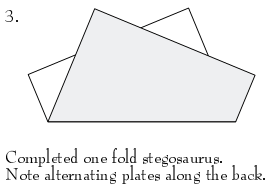
\includegraphics[width=2in]{figs/stego}}{figure}{fig:stego}
{From Wu's diagram}
Motivated by questions of how much paper is needed to fold a given origami model, 
we explore how folds can make a model bigger, in the sense that 
Joseph Wu's one-fold stegasaurus\footnote{An origami joke. 
\url{http://www.josephwu.com/Files/PDF/stegosaurus.pdf}}
cannot be covered by a copy of the square from which it is folded.

Other natural notions of making a model larger, namely area and perimeter,  
have been considered before.
It is clear that folding a piece of paper introduces overlap, so can
only decrease the area.  On the other hand, a rectangle or square can
have greater perimeter in a folded than an unfolded state---known 
as Arnold's ruble note or the Margulis napkin problem~\cite{a05,l03}. 
The folding techniques that increase perimeter, rumpling and
pleat-sinking, make very small (but thick)  models that are easily
covered by the original paper, however. 

Let's make our folding and covering problem more precise. 
All shapes will be closed 2-manifolds with
boundary (every interior point has a disk neighborhood, and every
boundary point has a half-disk), and be simply-connected (no holes). 
Distances within a shape will be measured along geodesic paths
within the shape.   For convex shapes, these are straight-line paths;
for non-convex, they may make turns at reflex points on the
boundary---that is, points having a half-disk with angle at least
180$^\circ$.  

One shape $P$ is said to cover $Q$ if some rotation and translation of $P$ contains
$Q$. The scale for $P$ to cover $Q$ is ths smallest $\alpha$ such that
$\alpha P$ covers $Q$.  This scale may be infinite. 
A fold of $P$ is \comm{fill in defn}.  We will state all of our claims
for flat folds, but can drop the ``flat'' if we understand covering to
mean covering the projection down into the plane. 

Our main general theorem upper and lower bounds the scale for a shape $P$ to cover its folds using
the following geometric parameters. 
An {\it incircle} for shape $P$ is a circle of maximum radius contained in
$P$; shape $P$ has one incircle radius, though it may have a set of
incircle centers.
A {\it diameter} of $P$ is a path that attains the maximum distance
between two points of $P$.   A {\it geodesic center} is a point in $P$ that
minimizes the maximum distance (the {\it geodesic radius}) to all
points of $P$. 
For any folding of $P$, every point remains within the
geometric radius of the geometric center, which gives an immediate
upper bound to the necessary scale factor.  
\begin{lemma}\label{lem:ub}
For a shape $P$ with incircle radius $r$ and geodesic radius~$R$, 
the scale~$\sigma$ to cover any flat-folded copy of $P$ is at most~$R/r$.
\end{lemma}
In \sref{genl}, we show
that the lower bound is within a constant factor.

\section{Single folds for specific shapes}

In this section we consider the scale factors for single folds of
squares, triangles, and disks.  
\comm{Playing it safe by not claiming for multiple folds.}

\begin{figure}[ht] 
\centering
\subfloat[Folded square with minimum bounding squares]{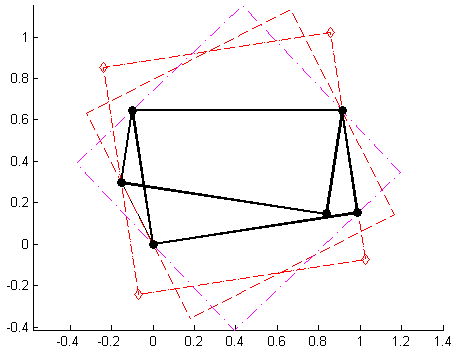
\includegraphics[width=2in]{figs/3boundingsq}
\label{fig:3boundingsq}}\hfil
%
\subfloat[Folded triangle with  min bounding triangle]{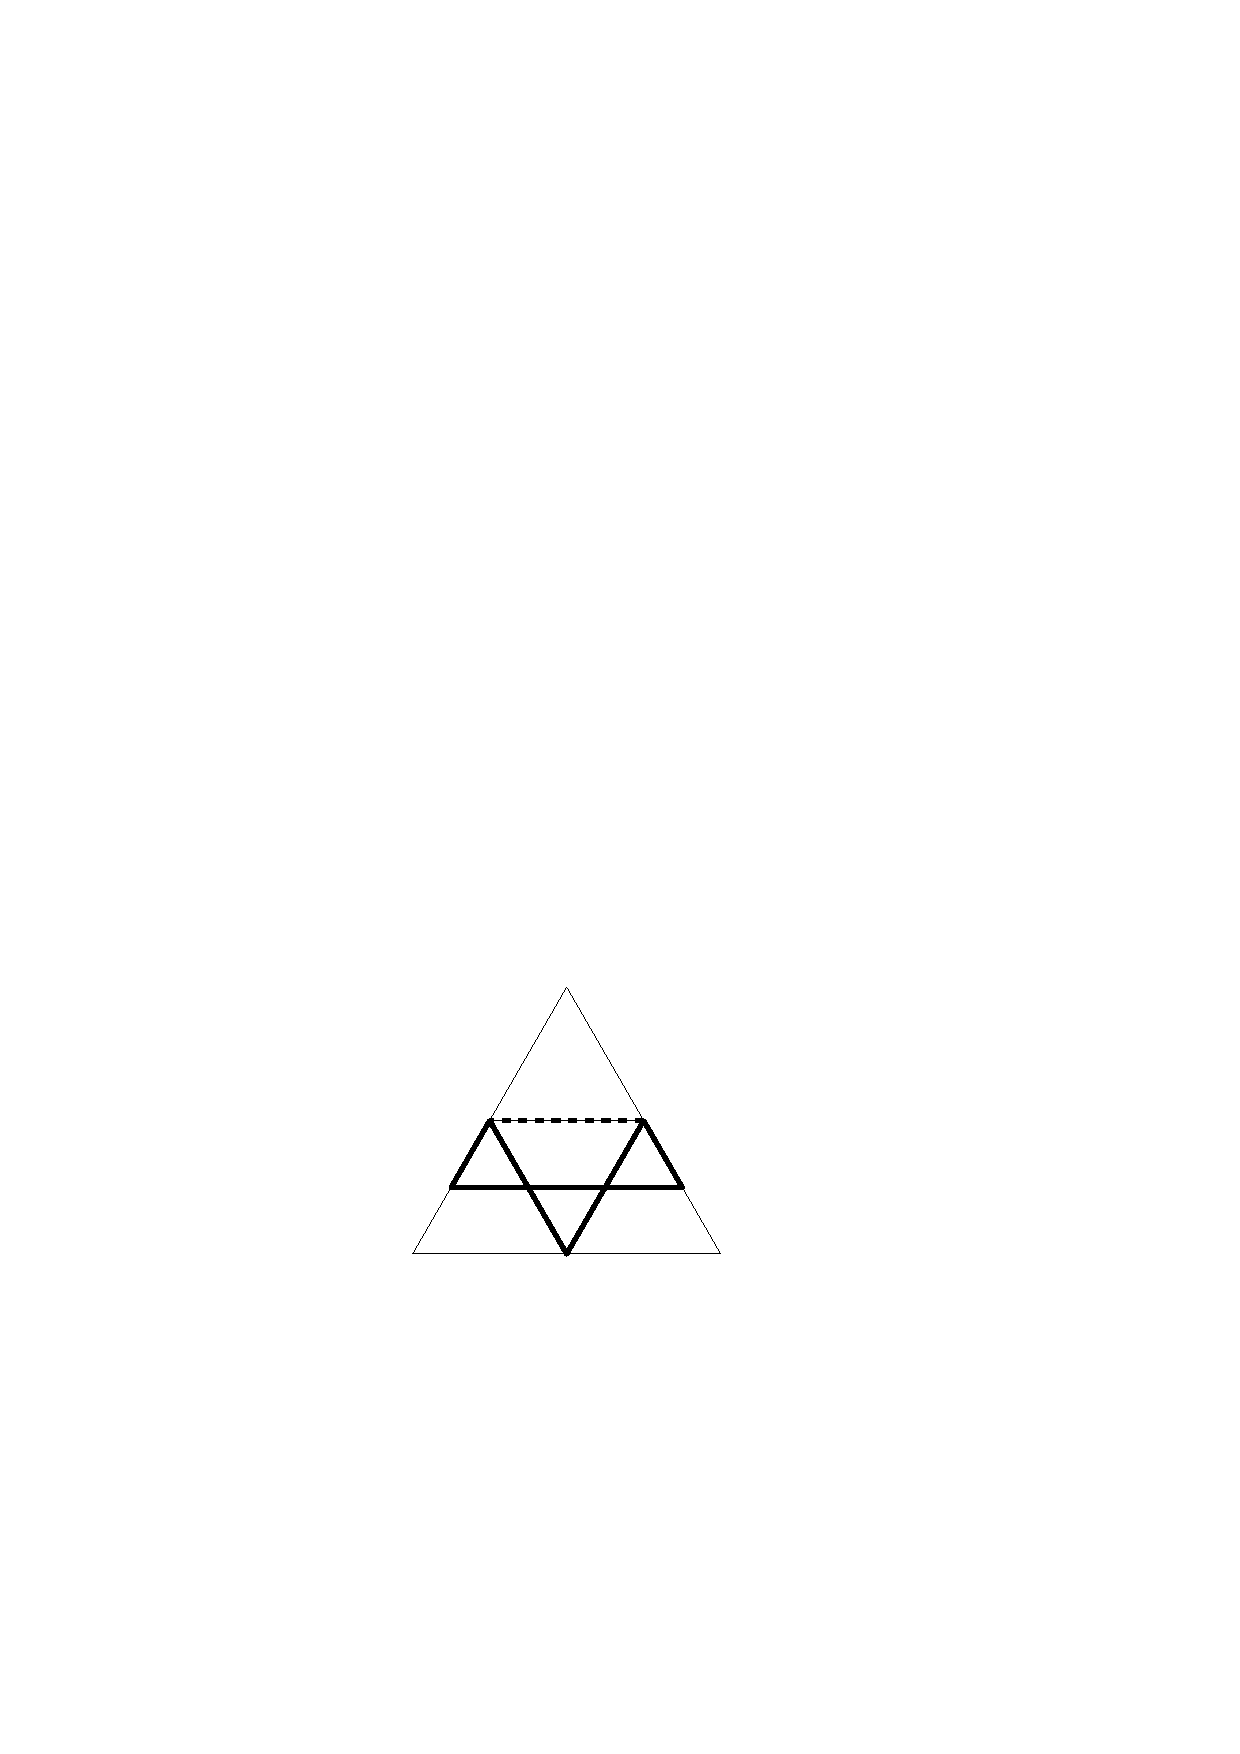
\includegraphics[width=1in]{figs/triangle}
\label{fig:triangle}}\hfil
%
\subfloat[Cut disk covers single folds, but not crimp]{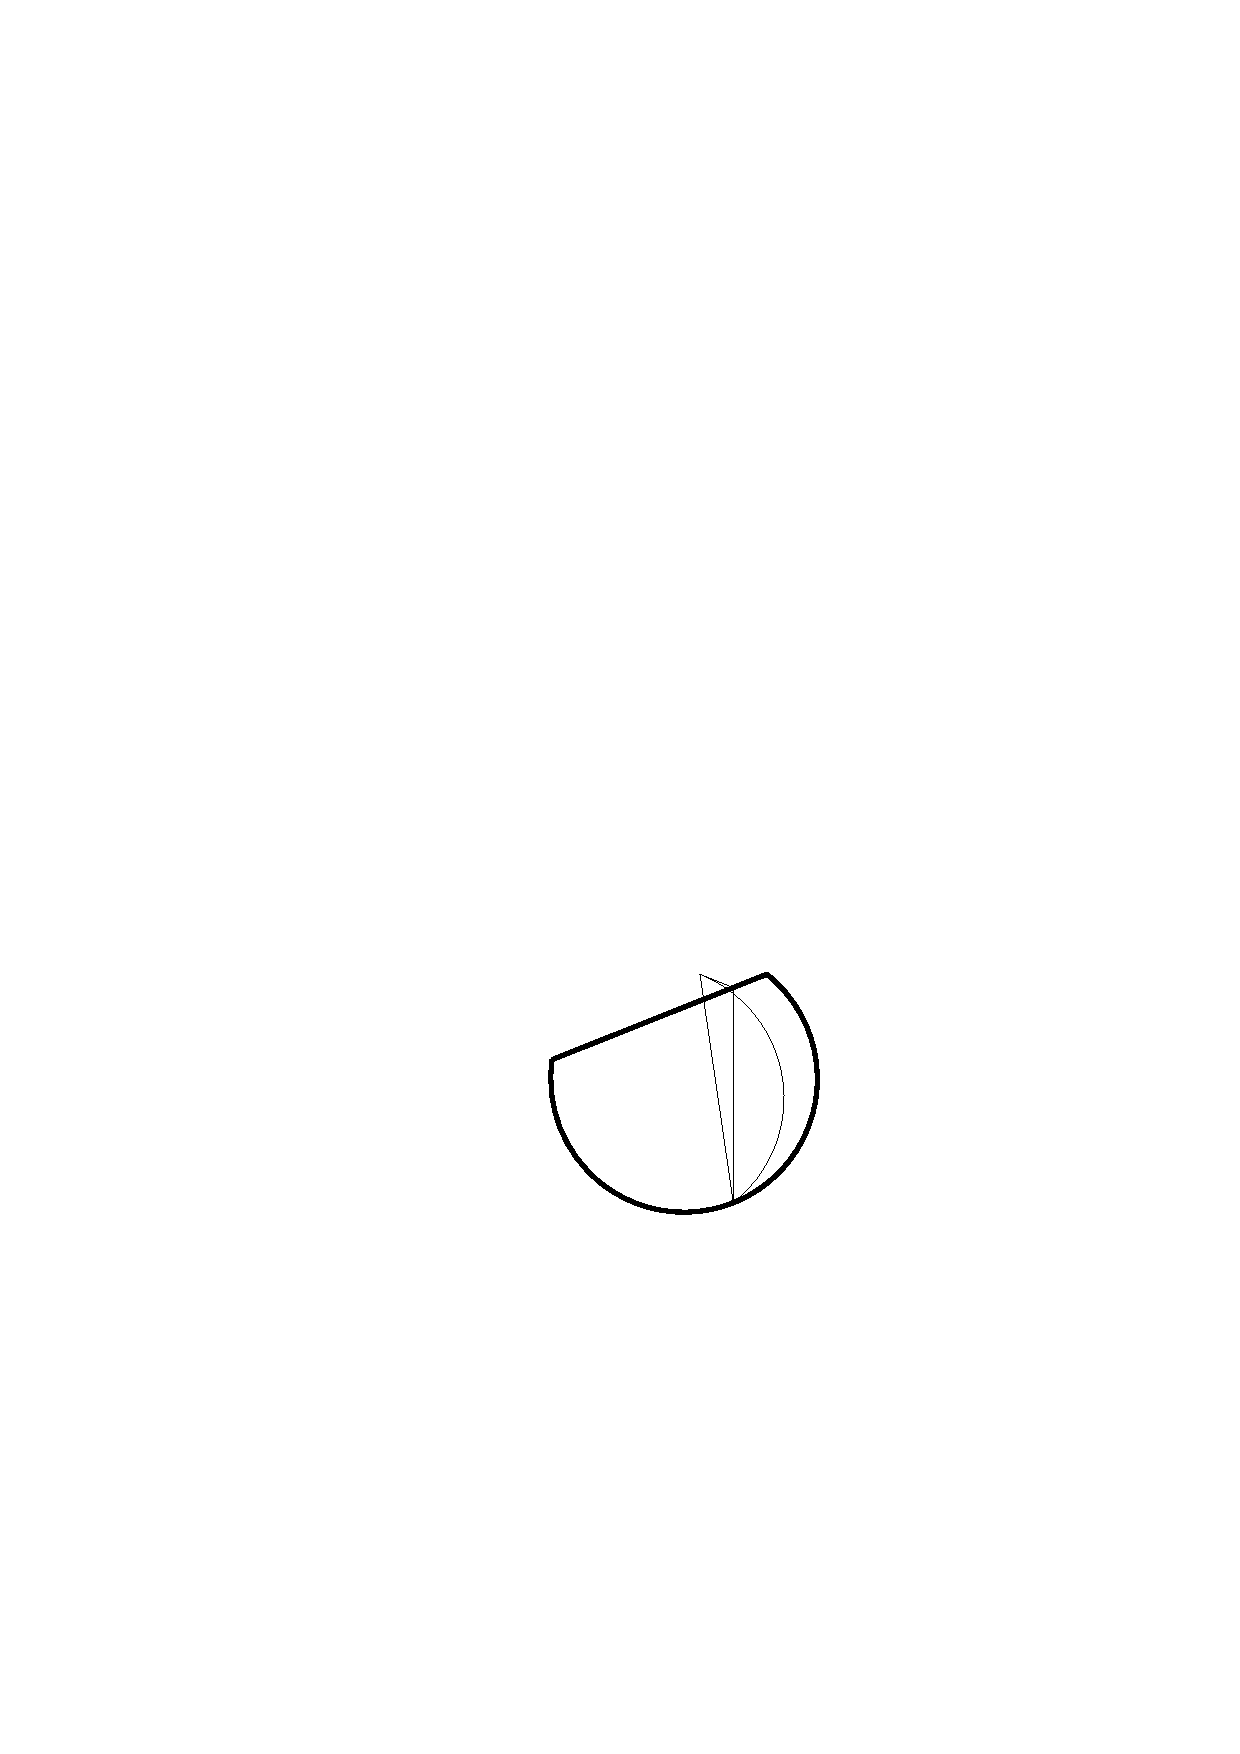
\includegraphics[width=.75in]{figs/cutdisk}
\label{fig:disk}}
\end{figure}
%
%\figbox[l]{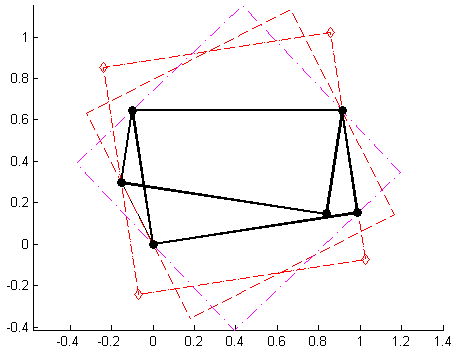
\includegraphics[width=2in]{figs/3boundingsq}}{figure}{fig:3boundingsq}{Folded square}
%\figbox[l]{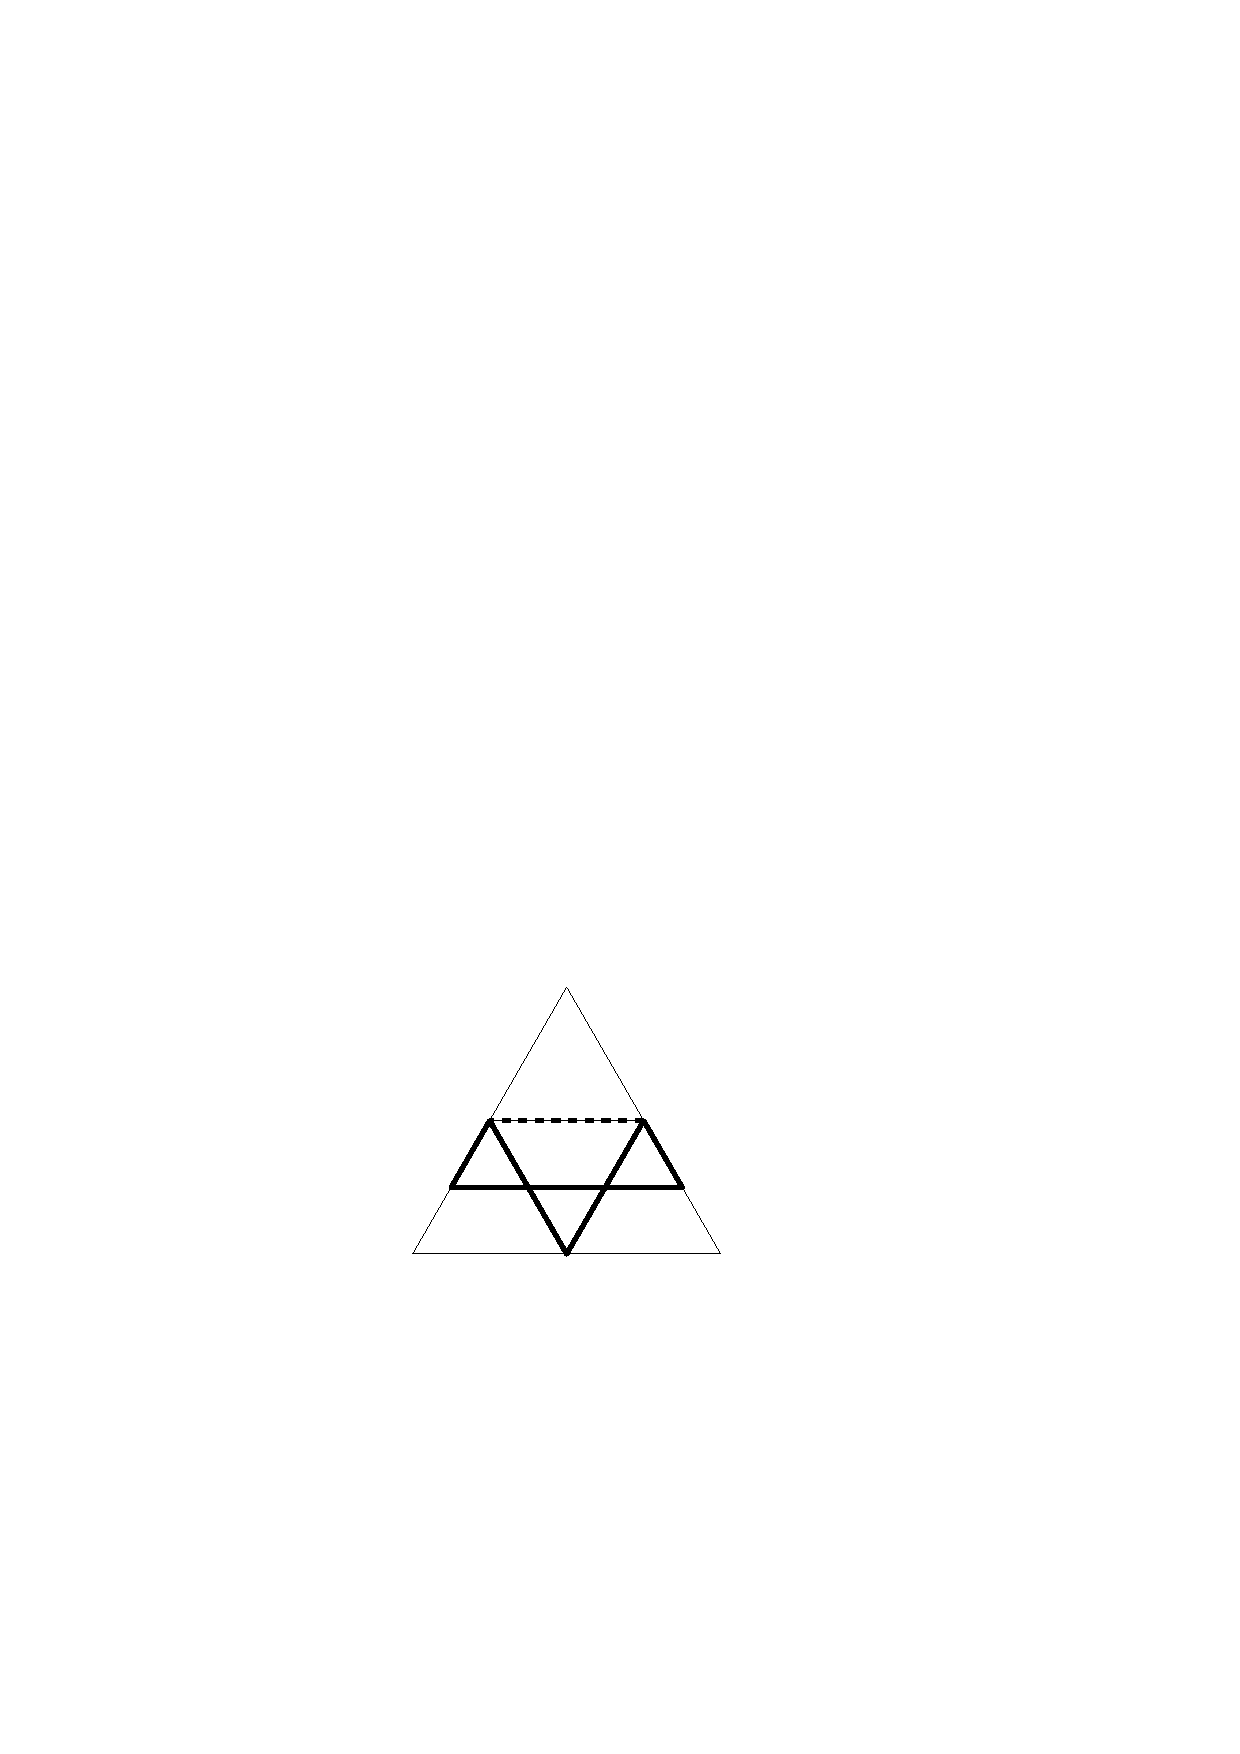
\includegraphics[width=1in]{figs/triangle}}{figure}{fig:triangle}{Folded triangle}
%\figbox[l]{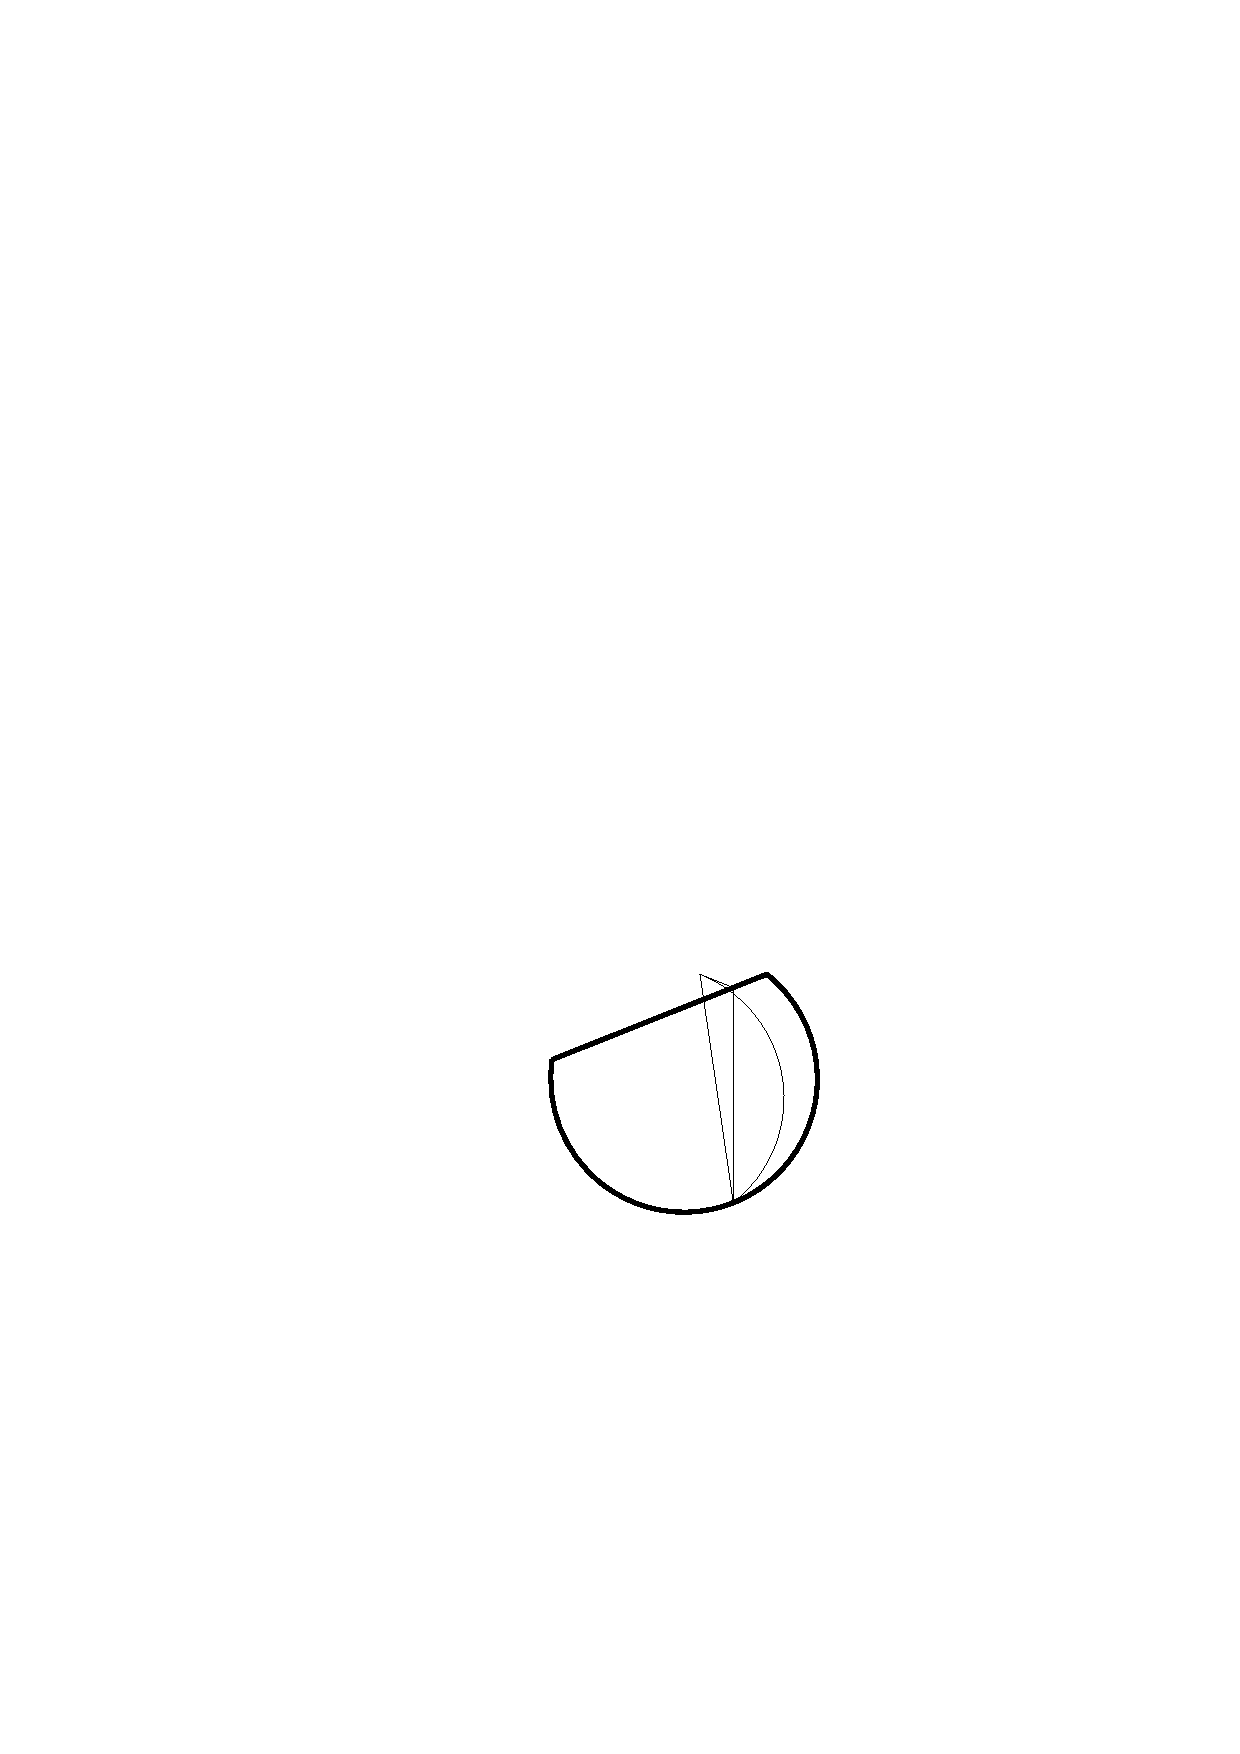
\includegraphics[width=1in]{figs/cutdisk}}{figure}{disk}{Cut   disk covers single folds, but not crimp.}

 {\bf Square:\/}  With a square, it is not difficult to numerically search for the
single fold that requires the maximum scale factor.  We used a
rotating calipers algorithm to compute the minimum bounding square,
which is defined by a side of the convex hull, or by a corner on each
side of the square.  (A clever construction of the square through four
points, which is unique when it exists, is problem 20 in Kovanova and
Radul's list of ``Jewish problems''~\cite{kr-jp-11}.)

 \fref{3boundingsq} shows the largest increase, which is just over
 10.5\%.  Initially we were surprised that it isn't the more symmetric
 stegosaurus fold---it even places one corner in the interior.  Its
 defining property is that it has three equal-size bounding squares,
 also shown: one along a side, one along a convex hull edge, and one
 through four points.

We prove \comm{in the full version} that this is the unique (up to
symmetry) fold that has three equal-sized bounding squares, and that
any fold with fewer than three distinct, equal-sized, bounding squares
can be adjusted to locally increase its scale factor.



 {\bf Triangle:\/} For an equilateral triangle, the bounding triangle is always
determined by an edge of the convex hull.  The largest scale factor
increase is 1/3, which is obtained by folding the tip over the line at
height 1/3 above the base.  
\comm{I probably have this wrong, since the notes say 27 percent. General triangles?}



 {\bf Disk:\/} 
Because the radius of a disk is also the incircle and the geodesic radius, 
a copy of a disk can cover any of its folds without scaling.  This sufficient
condition is not necessary, however; the shape $Q$ formed by removing
from a disk a sector of 120$\circ$ can also cover any of its single folds.
\comm{Add proof.} Note that this doesn't seem to
  work for two folds making the crimp shown.  Might if we add the arc that makes diameter
  $\sqrt 3/2$.

\section{Polygons}
I realized that the crimp we used for polygons also increases the
scale on the cut disk, so we have to decide what we will claim for
single folds and what we will claim for any folded state. 
  
\section{General bounds}\label{sec:genl}

In this section we prove the lower bound that goes with \lref{ub}.
\begin{lemma}\label{lem:lb}
For shape $P$ with incircle radius $r$, geodesic radius $R$, and
geodesic diameter $D$, there is a folded copy whose covering scale
factor $\sigma$ is satisfies $$\sigma\ge \max\{\frac{D}{2\pi
  r},\frac{R}{\sqrt 3\pi r}\}.$$
\end{lemma}
\begin{proof}
The basic idea is to find a path in $P$ that can be folded into a
large circle, which will then need to be covered by a scaled copy of
the incircle of $P$. 

\comm{JSS to provide details and better constants.}
\end{proof}

\section*{Acknowledgements}
We thank Godfried Toussaint and Erik Demaine for organizing the
Barbados 2013 workshop where this work was begun. 

%\vfil\eject
%\singlespace\small
%\bibliographystyle{plain}
%\bibliography{update,geom}
\begin{thebibliography}{1}
\bibitem{a05}
Arnold, V. I. (2005). 
Arnold's Problems. Berlin: Springer.
Problem 1956--1.
\bibitem{l03}
Lang, Robert J. (2003). Origami Design Secrets: Mathematical Methods
for an Ancient Art. A K Peters. pp. 315--319.
\bibitem{kr-jp-11}
Jewish Problems
Tanya Khovanova, Alexey Radul
 15 Oct 2011
http://arxiv.org/abs/1110.1556v2
\end{thebibliography}

\end{document}

Tabachnikov, Sergei (2007). "Book review of "Arnold's
problems"". Math. Intelligencer 29 (1):
49--52. http://dx.doi.org/10.1007%2FBF02984760
